
%-------------------------
% ATS-Friendly Resume in LaTeX
% Author: Nirmalya Mandal
%-------------------------

\documentclass[letterpaper,10pt]{article}

\usepackage[empty]{fullpage}
\usepackage{titlesec}
\usepackage{enumitem}
\usepackage[hidelinks]{hyperref}
\usepackage{fancyhdr}
\usepackage{fontawesome5}
\usepackage{graphicx}
\usepackage{xcolor}
\usepackage{geometry}
\usepackage{tabularx}
\usepackage{multicol}

% Page geometry
\geometry{
    left=0.4in,
    right=0.4in,
    top=0.4in,
    bottom=0.4in
}

\pagestyle{fancy}
\fancyhf{}
\fancyfoot{}
\renewcommand{\headrulewidth}{0pt}
\renewcommand{\footrulewidth}{0pt}

% URL style
\urlstyle{same}

% Hyperlink color
\hypersetup{
    colorlinks=true,
    linkcolor=blue,
    filecolor=blue,
    urlcolor=blue,
}

% Section formatting
\titleformat{\section}{
    \vspace{-4pt}\scshape\raggedright\large\bfseries
}{}{0em}{}[\color{black}\titlerule \vspace{-5pt}]

% Custom commands
\newcommand{\resumeItem}[1]{
    \item\small{#1 \vspace{-3pt}}
}

\newcommand{\resumeSubheading}[4]{
    \vspace{-3pt}\item
    \begin{tabular*}{0.97\textwidth}[t]{l@{\extracolsep{\fill}}r}
        \textbf{#1} & #2 \\
        \textit{\small#3} & \textit{\small #4} \\
    \end{tabular*}\vspace{-8pt}
}

\newcommand{\resumeProjectHeading}[2]{
    \item
    \begin{tabular*}{0.97\textwidth}{l@{\extracolsep{\fill}}r}
        \small#1 & #2 \\
    \end{tabular*}\vspace{-8pt}
}

\newcommand{\resumeSubItem}[1]{\resumeItem{#1}\vspace{-5pt}}

\renewcommand\labelitemii{$\vcenter{\hbox{\tiny$\bullet$}}$}

\newcommand{\resumeSubHeadingListStart}{\begin{itemize}[leftmargin=0.15in, label={}]}
\newcommand{\resumeSubHeadingListEnd}{\end{itemize}}
\newcommand{\resumeItemListStart}{\begin{itemize}}
\newcommand{\resumeItemListEnd}{\end{itemize}\vspace{-6pt}}

%-------------------------------------------
%%%%%%  RESUME STARTS HERE  %%%%%%%%%%%%%%%%%%%%%%%%%%%%

\begin{document}

%----------HEADING----------
\begin{center}
    \begin{minipage}[t]{0.15\textwidth}
        \vspace{0pt}
        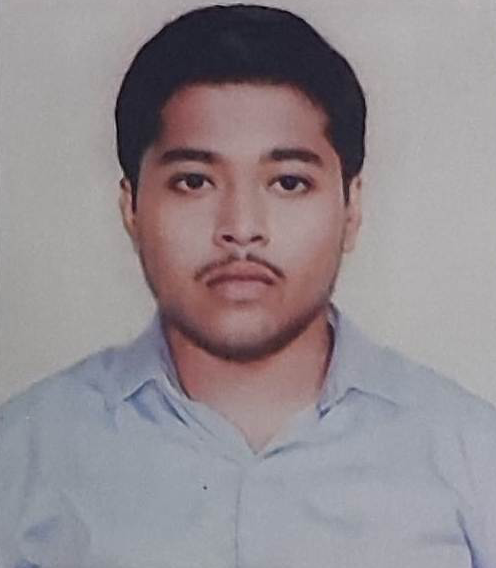
\includegraphics[width=1.1in,height=1.3in,keepaspectratio]{profile_photo}
    \end{minipage}%
    \hspace{0.5em}
    \begin{minipage}[t]{0.82\textwidth}
        \vspace{0pt}
        {\Huge \scshape \textbf{Nirmalya Mandal}} \\[10pt]
        % Contact Information
        \small
        {\color{black}\faPhone\ Phone:} \href{tel:+917001467098}{+91 7001467098} \hspace{1em}
        {\color{black}\faEnvelope\ Email:} \href{mailto:nirmalyamandal342@gmail.com}{nirmalyamandal342@gmail.com} \\[6pt]
        % Social Links
        {\color{black}\faGithub\ GitHub:} \href{https://github.com/DevNiru2704}{github.com/DevNiru2704} \hspace{0.5em}
        {\color{black}\faLinkedin\ LinkedIn:} \href{https://www.linkedin.com/in/nirmalya-mandal-9b2475313/}{linkedin.com/in/nirmalya-mandal-9b2475313} \\[4pt]
        {\color{black}\faCode\ LeetCode:} \href{https://leetcode.com/u/wQ6wdt3C20/}{leetcode.com/u/wQ6wdt3C20} \hspace{0.5em}
        {\color{black}\faGlobe\ Portfolio:} \href{https://www.nirmalyamandal.me}{nirmalyamandal.me}
    \end{minipage}
\end{center}

\vspace{-8pt}

%---------- PROFESSIONAL SUMMARY ----------
\section{Professional Summary}
\small{Driven Full Stack Developer with hands-on experience building production-grade web and mobile applications. Proficient in React, Next.js, React Native, Django, and FastAPI with expertise in deploying scalable solutions using Nginx, Docker, and cloud platforms. Experienced in integrating AI/ML capabilities including LLMs and RAG pipelines. A continuous learner with a deep hunger for knowledge, committed to mastering new technologies and best practices. Aspiring to grow into a highly skilled and respected developer known for technical excellence and impactful contributions.}

\vspace{-5pt}

%---------- EXPERIENCE ----------
\section{Experience}
    \resumeSubHeadingListStart
        \resumeSubheading
            {No Strategy Studios}{Remote}
            {Full Stack Developer}{Sep 2025 to Dec 2025}
            \resumeItemListStart
                \resumeItem{Developed premium e-commerce website for A Fashions (international leather manufacturer) using Next.js 16, TypeScript, and Tailwind CSS}
                \resumeItem{Collaborated with UI/UX designer to implement responsive design and interactive animations using Framer Motion}
                \resumeItem{Implemented enterprise security with multi-tier rate limiting, hCaptcha, XSS/CSRF prevention, and DDoS protection}
                \resumeItem{Achieved 100 SEO Lighthouse score with dynamic sitemap, Schema.org structured data, and 40+ organic keywords}
                \resumeItem{Deployed on GoDaddy VPS with Nginx reverse proxy, Certbot SSL certificates, and production server configuration}
            \resumeItemListEnd
            \vspace{5pt}
            \small{\textit{Client Website:} \href{https://www.afashions.net}{afashions.net}}

        \resumeSubheading
            {Doklink Services Private Limited}{Kolkata, India}
            {Full Stack Developer Intern}{Jun 2025 to Jul 2025}
            \resumeItemListStart
                \resumeItem{Developed and published emergency healthcare mobile app using React Native and Expo, available on Google Play Store}
                \resumeItem{Built RESTful APIs with Django REST Framework featuring JWT authentication, OTP verification, and Aadhaar integration}
                \resumeItem{Implemented real-time emergency bed booking with dynamic timing based on Haversine distance calculation}
                \resumeItem{Integrated Razorpay payment gateway and automated bed management with cron-based expiration handling}
                \resumeItem{Technologies: React Native, Expo, TypeScript, Django, PostgreSQL, JWT, Razorpay, Cloudinary}
            \resumeItemListEnd
            \vspace{5pt}
            \small{\textit{Play Store:} \href{https://play.google.com/store/apps/details?id=com.doklink.app}{play.google.com/store/apps/details?id=com.doklink.app}}
    \resumeSubHeadingListEnd

%---------- PROJECTS ----------
\section{Projects}
    \resumeSubHeadingListStart
        \resumeProjectHeading
            {\textbf{FloatChat} - \emph{AI-Powered Conversational Interface for Argo Ocean Data}}{}
            \resumeItemListStart
                \resumeItem{Built AI conversational platform for natural language queries on 23 years of Argo oceanographic data (79,934 records, 451 floats)}
                \resumeItem{Developed full-stack application with Next.js 15, TypeScript frontend and FastAPI Python backend with async support}
                \resumeItem{Integrated Mistral 7B LLM via HuggingFace for natural language to SQL generation with geographic/temporal intelligence}
                \resumeItem{Created interactive visualizations with 2D maps (Leaflet.js), 3D globe (Globe.gl), and depth profile charts}
                \resumeItem{Technologies: Next.js 15, TypeScript, FastAPI, Python, Mistral 7B, Supabase, Upstash Vector, LangChain, Leaflet.js, Globe.gl}
            \resumeItemListEnd
            \vspace{5pt}
            \small{\textit{Live:} \href{https://floatchat-chi.vercel.app}{floatchat-chi.vercel.app}  \textit{GitHub:} \href{https://github.com/DevNiru2704/floatchat}{github.com/DevNiru2704/floatchat}}
    \resumeSubHeadingListEnd

%---------- SKILLS ----------
\section{Skills}
    \begin{itemize}[leftmargin=0.15in, label={}]
        \small{\item{
            \textbf{Languages}{: JavaScript, TypeScript, Python, Java, C, C++, SQL, HTML5, CSS3} \\
            \textbf{Frontend}{: React, Next.js, React Native, Expo, Tailwind CSS, Framer Motion, Leaflet.js, Globe.gl} \\
            \textbf{Backend}{: Node.js, Express.js, Django, Django REST Framework, FastAPI, REST APIs} \\
            \textbf{Databases}{: PostgreSQL, Supabase, MongoDB, MySQL, Redis, Upstash Vector} \\
            \textbf{DevOps}{: Docker, Nginx, Certbot SSL, GoDaddy VPS, Linux Server Administration, CI/CD, Git} \\
            \textbf{AI/ML}{: LangChain, Mistral 7B, HuggingFace, RAG, Sentence Transformers, xarray, NetCDF} \\
            \textbf{Cloud \& Tools}{: Vercel, Cloudinary, ImageKit CDN, Razorpay, hCaptcha, JWT, OAuth}
        }}
    \end{itemize}

%---------- ACHIEVEMENTS ----------
\section{Achievements}
    \resumeItemListStart
        \resumeItem{\textbf{2nd Place at Amitron} - Internal Hackathon of Smart India Hackathon (SIH), Amity University Kolkata}
        % \resumeItem{\textbf{Competitive Programming:} LeetCode (X problems solved), Codeforces (Rating: XXXX) - \textit{Update with actual stats}}
        % \resumeItem{\textbf{Open Source Contributions:} Contributed to [Project Name] - \textit{Update with actual contributions}}
    \resumeItemListEnd

%---------- EDUCATION ----------
\section{Education}
    \resumeSubHeadingListStart
        \resumeSubheading
            {Amity University Kolkata}{Kolkata, India}
            {Bachelor of Technology, Computer Science and Engineering - CGPA: 8.10/10}{2023 to 2027}
        \vspace{2pt}
        \item
        \begin{tabular*}{0.97\textwidth}[t]{l@{\extracolsep{\fill}}r}
            \textbf{East West Model School, Talit} & Talit, India \\
            \textit{\small Higher Secondary (ISC Board) - 85.4\%} & \textit{\small 2023} \\
            \textit{\small Secondary (ICSE Board) - 85.67\%} & \textit{\small 2021} \\
        \end{tabular*}\vspace{-8pt}
    \resumeSubHeadingListEnd

%-------------------------------------------
\end{document}
